\section{Processi di Supporto}
\subsection{Documentazione}
\subsubsection{Scopo}
Ogni processo e attività per lo sviluppo del progetto dovrà essere documentata. Nella presente sezione verranno descritte regole e standard da seguire durante il processo di documentazione per l'intero ciclo di vita\textsuperscript{G} del software.

\subsubsection{Descrizione}
Vengono presentate decisioni e norme prescelte per:
\begin{itemize}
  \item Stesura;
  \item Verifica;
  \item Approvazione.
\end{itemize}

\subsubsection{Documenti prodotti}
I documenti prodotti sono:
\begin{itemize}
  \item \textbf{Norme di progetto}: documento interno che contiene norme e regole stabilite dal gruppo, che devono essere seguite per l’intera durata del progetto;
  \item \textbf{Glossario}: documento esterno dove sono presenti i termini tecnici usati nella documentazione con le loro definizioni, affinché non ci siano ambiguità e/o incongruenze;
  \item \textbf{Piano di progetto}: documento esterno con la pianificazione delle attività del progetto previste dal gruppo. Contiene la previsione dell’impegno orario dei singoli membri, il preventivo spese e i consuntivi di periodo;
  \item \textbf{Piano di qualifica}: documento esterno che descrive i criteri con cui si valuta la qualità;
  \item \textbf{Analisi dei requisiti}: documento esterno contenente requisiti e caratteristiche del prodotto finale;
  \item \textbf{Verbali}:
  \begin{itemize}
  		\item Interni: resoconti degli incontri del gruppo;
  		\item Esterni: resoconti degli incontri del gruppo con i committenti e/o il proponente.
	\end{itemize}
\end{itemize}

\subsubsection{Sistema software per la preparazione dei documenti}
Tutti i documenti prodotti dal gruppo verranno redatti usando il linguaggio di markup \LaTeX.

\subsubsection{Ciclo di vita di un documento}
Ogni documento passa per i seguenti step:
\begin{itemize}
  \item \textbf{Creazione}: il documento viene creato basandosi su un template comune;
  \item \textbf{Strutturazione}: il documento viene fornito di:
  \begin{itemize}
  		\item Registro delle modifiche;
  		\item Indice dei contenuti.
	\end{itemize}
  \item \textbf{Stesura}: il gruppo redige il documento adottando il metodo incrementale;
  \item \textbf{Revisione}: ogni sezione del corpo del documento è rivista da almeno un membro del gruppo che non sia il redattore della parte in verifica;
  \item \textbf{Approvazione}: se revisionato, il Responsabile di Progetto può stabilire che il documento è valido. Se approvato, può essere rilasciato.
\end{itemize}
Per semplificare le operazioni di verifica dovrà sempre essere reso disponibile il documento  completo (fino alla versione più attuale) in formato PDF.

\subsubsection{Struttura delle directory e dei files}
Per ogni documento si definisce la seguente struttura di directory:\\
\begin{forest}
  for tree={
    font=\ttfamily,
    grow'=0,
    child anchor=west,
    parent anchor=south,
    anchor=west,
    calign=first,
    edge path={
      \noexpand\path [draw, \forestoption{edge}]
      (!u.south west) +(7.5pt,0) |- node[fill,inner sep=1.25pt] {} (.child anchor)\forestoption{edge label};
    },
    before typesetting nodes={
      if n=1
        {insert before={[,phantom]}}
        {}
    },
    fit=band,
    before computing xy={l=15pt},
  }
[NomeDocumento
  [NomeDocumento.tex]
  [NomeDocumento.pdf]
  [Contenuto
    [Sezioni
        [Introduzione.tex]
        [Sezione1.tex]
        [Sezione2.tex]
    ]
    [Immagini
        [Immagine1.png]
        [Immagine2.jpeg]
    ]
    [Intro.tex]
    [RegistroModifiche.tex]
  ]
  [Struttura
    [Command.tex]
    [Impaginazione.tex]
    [Packages.tex]
  ]
]
\end{forest}\\

In particolare:
\begin{itemize}
\item \textbf{NomeDocumento.tex}: importa tutti le parti necessarie per comporre il documento finale;
\item \textbf{NomeDocumento.pdf}: versione del documento in formato PDF;
\item \textbf{Introduzione.tex}:  sezione introduttiva del documento, definisce lo scopo del prodotto e del documento, i riferimenti normativi e informativi e informazioni sul \textit{Glossario};
\item \textbf{Intro.tex}: contiene tutti i comandi per creare la prima pagina del documento;
\item \textbf{RegistroModifiche.tex}: contiene tutti i comandi per creare la tabella del registro delle modifiche;
\item \textbf{Command.tex}: contiene tutti i comandi aggiuntivi creati dal gruppo;
\item \textbf{Impaginazione.tex}: definisce alcune istruzioni per l'impaginazione e si occupa di creare header e footer del documento;
\item \textbf{Packages.tex}: contiene tutti i pacchetti aggiuntivi e necessari per la compilazione.
\end{itemize}


\subsubsection{Struttura di un documento}
\paragraph{Prima pagina}
La prima pagina è composta da:
\begin{itemize}
  \item \textbf{Logo del gruppo};
  \item \textbf{Titolo del documento};
  \item \textbf{Informazioni varie del documento}:
      \begin{itemize}
      \item \textbf{Versione corrente};
      \item \textbf{Approvatori}: indica chi ha approvato il documento. Se non presente, indica che il documento non è ancora stato approvato;
      \item \textbf{Data approvazione};
      \item \textbf{Redattori}: indica chi si è occupato della stesura del documento;
      \item \textbf{Verificatori}: indica chi si è occupato della verifica del documento;
      \item \textbf{Uso}: indica se il documento è dedicato a uso interno o esterno;
      \item \textbf{Distribuzione}: indica a chi viene distribuito il documento;
        \end{itemize}
\item \textbf{Indirizzo e-mail del gruppo}.
\end{itemize}

\paragraph{Registro delle modifiche}
Ogni documento ha il suo registro modifiche che tiene traccia di tutte le modifiche importanti del documento durante il suo ciclo di vita.
Sotto forma di tabella, riporta:
  \begin{itemize}
  		\item Versione del documento dopo la modifica;
  		\item Data della modifica;
  		\item Nome dell’autore della modifica;
  		\item Ruolo dell’autore al momento della modifica;
  		\item Descrizione breve della modifica;
  		\item Nome della persona che si è occupata di verificare la modifica.
	\end{itemize}

Inoltre, nella descrizione di ciascuna modifica viene indicato anche il paragrafo interessato con questa convenzione: 
\begin{itemize}
    \item \textbf{\S{}}: indica un solo paragrafo;
    \item \textbf{\S{}\S{}}: indica l'intervallo di paragrafi su cui sono state apportate le modifiche fatte.
\end{itemize}

\paragraph{Indice}
Presente dopo il registro delle modifiche, l’indice permette di avere una visione completa del documento e di individuare le varie parti, ogni voce è un collegamento ipertestuale alla parte del documento in cui viene trattata.

\paragraph{Struttura delle pagine}
Ogni pagina, a eccezione della prima, è formata da questi elementi:
  \begin{itemize}
  		\item In alto a sinistra si trova una miniatura a colori del logo del gruppo;
  		\item In alto a destra è presente il titolo del documento;
  		\item Sotto i due elementi appena elencati una linea nera continua li separa dal contenuto della pagina;
  		\item Il contenuto della pagina;
  		\item Sul lato destro del piè di pagina è indicato il numero della pagina corrente.
	\end{itemize}
	
\paragraph{Verbali}
I verbali applicano le stesse norme strutturali degli altri documenti con la differenza che non sono soggetti a versionamento\textsuperscript{G}. Ogni verbale sia interno che esterno dovrà contenere:
\begin{itemize}
\item Motivo della riunione;
\item Luogo della riunione;
\item Data della riunione;
\item Orario di inizio e fine riunione;
\item Partecipanti della riunione;
\item Resoconto della riunione;
\item Riepilogo delle decisioni, dove si riporta in tabella le decisioni prese dal gruppo durante l’incontro;
\item Riepilogo dei ticket, dove si riportano i ticket creati successivamente all'incontro.
\end{itemize}  		

\subsubsection{Normativa tipografica}
\paragraph{Nomi dei documenti}
La struttura generale del nome è la seguente: \\ \\
\centerline{\textbf{[NomeDocumento]-v[X].[Y].[Z]}}\\
in particolare:
\begin{itemize}
\item \textbf{[NomeDocumento]} inizia sempre con la lettera maiuscola. Se presenti più parole, queste saranno attaccate ma distinguibili dalla lettera maiuscola (convenzione \textit{"CamelCase"}\textsuperscript{G});
\item \textbf{v[X].[Y].[Z]} rappresenta la versione corrente del documento seguendo lo schema di versionamento presentato in §3.2.3;
\end{itemize}
I verbali, in quanto non soggetti a versionamento avranno una struttura del nome diversa, ovvero:\\ \\
\centerline{\textbf{Verbale[Tipologia]-[YYYY].[MM].[DD]}} \\
dove:
\begin{itemize}
\item \textbf{[Tipologia]} intende il tipo del verbale, può essere \textbf{Interno} o \textbf{Esterno};
\item \textbf{[YYYY].[MM].[DD]} indica la data in cui è avvenuto l'incontro.
\end{itemize}


\paragraph{Stile di testo}
Gli stili di testi adottati nei documenti sono:
\begin{itemize}
\item \textbf{Grassetto}: per titoli, sottotitoli, e altri termini ritenuti importanti dal redattore;
\item \textbf{Maiuscolo}: per acronimi e iniziali di nomi propri, dei documenti o dei paragrafi;
\item \textbf{Corsivo}: per nomi propri dei membri del gruppo, committenti e proponente e per i nomi dei documenti.
\end{itemize}


\paragraph{Termini di glossario}
I termini che possono risultare ambigui e/o incongruenti sono contrassegnati con una \textsuperscript{G} alla loro prima occorrenza nella sezione d’interesse. Questi termini sono riportati con il loro significato in un documento esterno, il \textit{Glossario}.

\paragraph{Elementi testuali}
I redattori devono seguire le seguenti regole stilistiche:
\begin{itemize}
\item \textbf{Elenchi puntati}: un elenco puntato utilizzerà il simbolo • (pallino). Un successivo annidamento utilizzerà il simbolo - (trattino) e un altro ancora un asterisco (*). Se si tratta di un elenco numerato, i quattro livelli di enumerazione sono ordinati con i numeri arabi divisi da un punto fermo. Ogni voce dell’elenco inizia con una lettera maiuscola e termina con un punto e virgola, tranne l'ultima voce che termina con un punto;

\item \textbf{Formati di data}: Le date usano il formato \textbf{[YYYY]-[MM]-[DD]} dove:
    \begin{itemize}
    \item \textbf{[YYYY]} corrisponde all’anno;
    \item \textbf{[MM]} corrisponde al mese;
    \item \textbf{[DD]} corrisponde al giorno.
    \end{itemize}

\item \textbf{Orario}: gli orari usano il formato \textbf{[HH]:[MM]} dove:
    \begin{itemize}
    \item \textbf{[HH]} rappresentano le ore;
    \item \textbf{[MM]} rappresentano i minuti.
    \end{itemize}

\item \textbf{Sigle}: Tutte le sigle hanno le iniziali di ogni parola maiuscola tranne preposizioni, congiunzioni e articoli. Le sigle utilizzate sono:
    \begin{itemize}
    \item Relative ai documenti:
        \begin{itemize}
        \item \textbf{Analisi dei Requisiti}: AdR;
        \item \textbf{Piano di Progetto}: PdP;
        \item \textbf{Piano di Qualifica}: PdQ;
        \item \textbf{Glossario}: G;
        \item \textbf{Norme di Progetto}: NdP;
        \item \textbf{Verbali Interni}: VI;
        \item \textbf{Verbali Esterni}: VE.
        \end{itemize}
    
    \item Relative ai ruoli di progetto:
        \begin{itemize}
        \item \textbf{Responsabile di Progetto}: RE;
        \item \textbf{Progettista}: PT;
        \item \textbf{Analista}: AN;
        \item \textbf{Amministratore}: AM;
        \item \textbf{Programmatore}: PR;
        \item \textbf{Verificatore}: VE.
        \end{itemize}
    \end{itemize}
\end{itemize}

\paragraph{Elementi grafici}
Le regole per quanto riguarda l’uso di elementi grafici sono:
\begin{itemize}
\item \textbf{Immagini}: le figure presenti sono centrate rispetto al testo e accompagnate da didascalia;
\item \textbf{Diagrammi UML}: verranno inseriti nel documento tramite delle immagini.
\end{itemize}

\subsubsection{Metriche}
Per la valutazione dei documenti prodotti del processo di documentazione, verrà applicata la seguente metrica di prodotto:
\begin{itemize}
\item \textbf{MQP01 Indice di Gulpease} \\
È un indice di leggibilità di un determinato testo. Calcola la lunghezza delle parole e delle frasi rispetto al numero totale delle lettere, per fare ciò considera: la lunghezza della parola e la lunghezza della frase rispetto al numero delle lettere. Il valore è un numero intero compreso tra 0 e 100.
La formula è:
\begin{itemize}
  \item[] \[IDG =  89 + \frac{300 * NDF - 10 * NDL}{NDP};\]
  \item NDF = Numero dei frasi;
  \item NDL = Numero di lettere;
  \item NDP = Numero di parole.
  \end{itemize}
\end{itemize}

\subsubsection{Strumenti}
Gli strumenti dedicati alla stesura sono:
\begin{itemize}
\item \textbf{\LaTeX}: linguaggio compilato basato sul programma di composizione tipografica Tex;
\item \textbf{Texmaker}: l’editor per la stesura dei documenti;
\item \textbf{Overleaf}: editor per la stesura dei documenti basato sul cloud\textsuperscript{G} ;
\item \textbf{Draw.io}: sito online per la creazione di grafici UML;
\item \textbf{GanttProject}: programma usato per la realizzazione di diagrammi di Gantt\textsuperscript{G}.
\end{itemize}

\subsection{Gestione della configurazione}
\subsubsection{Scopo}
Lo scopo è di gestire e controllare la produzione di documenti e codice in maniera sistematica. Per ogni oggetto sottoposto a configurazione viene garantito il versionamento e controllo sulle modifiche per permettere il mantenimento dell'integrità del prodotto. 

\subsubsection{Descrizione}
Vengono raggruppati e organizzati tutti i mezzi usati per la configurazione degli strumenti designati alla produzione di documenti e codice, per poter gestire struttura e la disposizione dei file all’interno del repository\textsuperscript{G} e anche  quelli per versionamento e coordinamento.

\subsubsection{Versionamento}
Per poter capire lo stato di avanzamento di un prodotto delle attività del progetto è necessario un identificatore. Il formato del codice di versione utilizzato è \\ \\
\centerline{\textbf{v[X].[Y].[Z]}} \\ \\
dove :
\begin{itemize}
\item \textbf{X} indica il rilascio pubblico e corrisponde ad una versione approvata dal Responsabile di Progetto. La numerazione parte da 0;
\item \textbf{Y} indica una revisione complessiva del prodotto per verificare che, dopo una modifica, il prodotto sia ancora coeso e consistente. La numerazione parte da 0 e si azzera ad ogni incremento di X;
\item \textbf{Z} viene incrementato ad ogni modifica con relativa verifica. La numerazione parte da 0 e si azzera ad ogni incremento di X o Y.
\end{itemize}

\paragraph{Strumenti}
Per il versionamento si è scelto di utilizzare un repository GitHub, che, a sua volta, implementa il software di controllo versione distribuito Git.

\subsubsection{Repository per la documentazione}
\paragraph{Struttura}
Il repository utilizzato dal gruppo per il versionamento dei documenti, denominato \textbf{Documenti}, contiene una directory per ogni documento denominata NomeDocumento, la cui struttura è approfondita in §3.1.6.
Il repository è suddiviso in più branch così definiti:
\begin{itemize}
\item \textbf{main}: il branch principale, che contiene l'ultima versione verificata di ogni documento;
\item \textbf{NomeDocumento}: uno per ogni documento, è dove il documento vive e viene attivamente stilato dai membri del gruppo.
\end{itemize}

\paragraph{Modifiche}
Viene fortemente sconsigliato fare commit\textsuperscript{G} direttamente sul branch\textsuperscript{G} \textbf{main}, poiché porterebbe ad un elevato rischio di incongruenze e merge conflicts\textsuperscript{G}. Potrà essere modificato solo tramite il meccanismo di pull request\textsuperscript{G} con verifica obbligatoria, in modo da garantire che sia sempre presente una versione verificata e corretta del documento, anche se incompleta.
Nel branch \textbf{NomeDocumento} invece ogni membro può fare commit a patto che siano relative solo al documento specificato. Ogni commit, dove possibile, deve referenziare la issue\textsuperscript{G} da cui è derivata e quindi, in generale, potranno effettuare modifiche sul branch solo gli assegnatari di issue che trattano quel documento specifico. Per quanto riguarda cambiamenti minimali (punteggiatura, errori ortografici, ecc.) è permessa la modifica autonoma da parte di qualsiasi membro del gruppo e non è necessario referenziare nessuna issue.
La gestione delle issue (ticket) viene trattata in §4.1.4.2.


\subsubsection{Repository per il codice}
\paragraph{Struttura}
Vengono utilizzati 3 repository per il versionamento del codice relativo al prodotto software. In particolare:
\begin{itemize}
	\item \textbf{CrawlingService}: contiene il codice Python per il microservizio che si occupa dell'attività di estrazione dei dati tramite crawling;
	\item \textbf{CrawlingService}: contiene il codice Python per il microservizio che si occupa dell'analisi dei dati estratti e fornisce la maggior parte delle API al frontend;
	\item \textbf{FrontendSWEET}: contiene il codice Javascript/HTML/CSS che compone il frontend del prodotto software.
\end{itemize}
Viene utilizzato il \textit{Feature Branch Workflow}\textsuperscript{G}, dove ogni aggiunta di codice significativa viene eseguita in un branch secondario, le modifiche verrano poi trasferite al branch principale tramite il meccanismo di pull request.

I repository quindi sono suddivisi in più branch, in generale:
\begin{itemize}
\item \textbf{main}: il branch principale, che contiene l'ultima versione funzionante del codice;
\item \textbf{Feature branch}: uno per ogni feature\textsuperscript{G}, dove uno o più, membri lavorano al codice, al termine verrà fatto il merge\textsuperscript{G} nel main branch.
\end{itemize}

Non vengono definite regole specifiche circa la nomenclatura dei feature branch, che quindi sono a discrezione dei singoli programmatori. 
L'unico principio guida è che devono essere concisi e esplicativi.

\paragraph{Modifiche}
Vengono impedite le commit sul branch main, perchè, soprattutto per il codice, potrebbero portare a conflitti potenzialmente disastrosi. Secondo il Feature Branch Workflow, per ogni feature verrà creato un branch, dove uno o più programmatori lavoreranno al codice, una volta terminato, verrà fatta pull request di merge la main, e dopo verifica, verrà accettata.
Ogni commit deve, quando possibile, contenere un riferimento alla issue che l'ha resa necessaria.\\
I singoli gruppi di sviluppo si impegnano a mantenere una versione il più possibile corretta  completa del software nel branch main.


\subsection{Gestione della qualità}
\subsubsection{Scopo}
Lo scopo del processo di gestione della qualità è di assicurare che i requisiti di qualità individuati dagli stakeholder e le esigenze espresse dal proponente vengano rispettate dai prodotti e processi da sviluppare.

\subsubsection{Descrizione}
Il \textit{Piano di Qualifica} è il documento dedicato alla gestione della qualità. In esso sono descritti metriche e standard con le quali misurare e valutare la qualità di prodotti e processi.  

\subsubsection{Attività di processo}
Si possono individuare tre attività principali nel processo di gestione della qualità:
\begin{itemize}
\item \textbf{Pianificazione}: definire obiettivi di qualità, le strategie per raggiungerli e le risorse necessarie; 
\item \textbf{Valutazione}: applicare quanto pianificato, misurando i risultati;
\item \textbf{Reazione}: analizzando i risultati ottenuti con lo scopo di attuare miglioramenti o sanare situazioni non desiderate.
\end{itemize}

\subsubsection{Controllo di qualità}
Per essere sicuri di arrivare alla qualità desiderata, ogni membro deve essere in grado di:
\begin{itemize}
\item Comprendere gli obiettivi da raggiungere;
\item Individuare eventuali errori;
\item Stimare in termini di valore, dimensione e complessità le task;
\item Produrre risultati concreti e quantificabili;
\item Miglioramento costante della propria formazione;
\item Utilizzo del sistema di ticket offerto da Github;
\item Svolgimento di \textit{Code refactoring};
\item Rispetto degli standard adottati e delle norme definite in questo documento.
\end{itemize}

\subsubsection{Code refactoring}
L'attività di \textit{code refactoring} migliora la struttura, leggibilità, manutenibilità e performance del codice senza alterarne il funzionamento e introdurre delle recessioni. Aiuta inoltre nell'individuazione di errori.
In generale è uno dei compiti del programmatore, e va effettuato solo dopo che il codice ha passato tutti i test e le metriche definite nel \PdQ. 
Importante è sfruttare alcune funzionalità aggiuntive degli IDE utilizzati, che permettono un'automatizzazione di alcuni aspetti del \textit{code refactoring}.

\subsubsection{Denominazione metriche e obiettivi}
Per la denominazione delle metriche è stato adottato il formato: \\ \\
\centerline{\textbf{M[Tipologia][Numero]}} \\ \\
mentre per la denominazione degli obiettivi di qualità è stato adottato il formato: \\ \\
\centerline{\textbf{Q[Tipologia][Numero]}} \\ \\
dove:
\begin{itemize}
\item \textbf{[Tipologia]}: indica la tipologia a cui si riferisce la metrica, può assumere tre valori:
    \begin{itemize}
    \item \textbf{PC}: relativa ai processi; 
    \item \textbf{QP}: relativa ai prodotti;
    \item \textbf{TS}: relativa ai test.
    \end{itemize}
\item \textbf{[Numero]}: indica il numero progressivo della metrica, parte da 1.
\end{itemize}	

\subsection{Verifica}
\subsubsection{Scopo}
Lo scopo è definire come attuare il processo di verifica, per accertarsi che non ci siano errori durante lo sviluppo del prodotto, che la redazione della documentazione e che i requisiti in oggetto vengano rispettati. 

\subsubsection{Descrizione}
La verifica viene applicata ad ogni processo in esecuzione. Per il processo di verifica ci si affida all'analisi e ai test. L'analisi si divide in due tipologie:
\begin{itemize}
\item \textbf{Statica}: non richiede l'esecuzione dell'oggetto in verifica, perciò è applicabile ad ogni prodotto. Accerta il rispetto della normativa e l'assenza di errori studiando il codice sorgente o la documentazione;
\item \textbf{Dinamica}: richiede l'esecuzione dell'oggetto in verifica, applicabile perciò solo al codice. Fa largo uso di test.
\end{itemize}

\subsubsection{Verifica della documentazione}
Si utilizza un'analisi statica. Si possono utilizzare strumenti automatici oppure si può fare a mano (desk check) attraverso due metodi:
\begin{itemize}
\item \textbf{Walkthrough}: che consiste in un controllo completo del documento tramite una lettura ad ampio spettro;
\item \textbf{Inspection}: che consiste in un controllo specifico tramite una lettura mirata del documento.
\end{itemize}

\paragraph{Walkthrough}
Attività svolta dal \VE{}, viene di norma adottata nelle fasi iniziali. Risulta essere molto onerosa e quindi va ridotto l'uso il prima possibile. Nel caso del nostro gruppo, questo metodo verrà adottato fino a che non sarà disponibile una lista di controllo.

\paragraph{Inspection}
Attività svolta dal \VE{}, sfrutta una lettura mirata per trovare gli errori tramite una lista di controllo, compilata seguendo gli errori più comuni nelle varie verifiche in modalità Walkthrough. Rispetto la tecnica Walkthrough, questo metodo è meno oneroso e da preferire, verrà utilizzato dal nostro gruppo quando sarà disponibile una lista di controllo esaustiva.


\subsubsection{Verifica del codice}
Il codice verrà verificato attraverso test automatici, e tramite le metriche e misurazioni varie definite all'interno del \PdQ. 
In particolare il codice dovrà rispettare le seguenti regole:
\begin{itemize}
\item Dovrà essere direttamente derivato dalla progettazione o dai requisiti;
\item Dovrà essere testabile, corretto e leggibile.
\end{itemize}

\paragraph{Analisi statica}
L'analisi statica si controlla la bontà del codice, senza eseguirlo, sia dal punto di vista della correttezza che del rispetto delle norme di buona programmazione definite dal gruppo (vedi §2.4.3.1). Il gruppo ha deciso di sfruttare alcuni plugin specifici degli IDE utilizzati, che effettuano un analisi statica del codice in automatico, permettendo di risolvere molti errori il prima possibile.

\paragraph{Analisi dinamica}
L'analisi dinamica si controlla la presenza o meno di bug durante l'esecuzione del software prodotto. Vengono sfruttati i test specifici prodotti per il codice, questo permette di verificare il corretto funzionamento o individuare criticità o scostamenti dai risultati attesi.

In generale i test dovranno essere:
\begin{itemize}
	\item ripetibili;
	\item isolati;
	\item veloci;
	\item fornire informazioni sui risultati dell’esecuzione.
\end{itemize}

\paragraph{Test}
I test sono l'attività fondamentale dell'analisi dinamica. Servono per dimostrare che il programma funzioni e svolga ciò per cui è stato sviluppato. I test si dividono in quattro categorie, in base all'oggetto in verifica e allo scopo: 
\begin{itemize}
\item \textbf{Test d'unità}: verificano una singola unità di codice, la più piccola parte che ha senso verificare (es. singola procedura);
\item \textbf{Test d'integrazione}: verificano la correttezza delle interfacce. Si vuole stabilire il corretto funzionamento delle varie componenti, una volta passato il test d'unità, aggregandole man mano e verificando il funzionamento nel complesso;
\item \textbf{Test di sistema}: verifica l'applicazione nella sua interezza. Venendo dopo il test d'integrazione, lo scopo è verificare che le componenti non solo sono compatibili, ma che lo scambio di dati tra interfacce e le varie interazioni siano conformi. Inoltre, così si controlla che i requisiti siano stati soddisfatti;
\item \textbf{Test di regressione}: verifica l'applicazione dopo aver apportato modifiche al sistema. Lo scopo è controllare nuove funzionalità non testate e, al tempo stesso, garantire che il codice già presente e testato in precedenza non subisca alterazioni al suo comportamento.
\end{itemize}

\paragraph{Nominazione dei test}
Ogni test verrà identificato con un codice: \\ \\
\centerline{\textbf{T[Tipologia][Componente][Id]}} \\ \\
In particolare:
\begin{itemize}
\item \textbf{Tipologia}: Indica la tipologia del test:
	\begin{itemize}
	\item \textbf{U}: Unità;
	\item \textbf{I}: Integrazione;
	\item \textbf{S}: Sistema;
	\item \textbf{R}: Regressione;
	\item \textbf{V}: Validazione (trattati in §3.5.4.1).
	\end{itemize}
	
\item \textbf{Componente}: Rappresenta la singola componente a cui i test si riferiscono:
	\begin{itemize}
	\item \textbf{F}: Frontend;
	\item \textbf{CS}: Crawling service;
	\item \textbf{RS}: Ranking service.
	\end{itemize}
	Viene applicato solo per i test di unità. 	
	
\item \textbf{Id}: codice numerico per identificare i test dello stesso tipo, parte da 1.

\end{itemize}


\subsubsection{Verifica dei requisiti}
Vengono applicate Walkthrough e Inspection per controllare validità e coerenza con quanto dichiarato e descritto all'interno dell'\textit{Analisi dei Requisiti}, oltre a quanto dichiarato al proponente.


\subsubsection{Strumenti}
Gli strumenti utilizzati dal gruppo per la verifica automatica del codice sono:
\begin{itemize}
\item \textbf{Jest}: Framework di test JavaScript e TypeScript gestito da Facebook;
\item \textbf{unittest}: Framework di test Python, integrato nelle librerie standard;
\item \textbf{Code Climate}: Plugin per Atom che integra molti strumenti di analisi statica nell'IDE stesso;
\item \textbf{Code Inspections}: Funzionalità integrata di PyCharm che permette di eseguire analisi statica del codice, con un buon livello di personalizzazione. 
\end{itemize}

\subsubsection{Metriche}
Per la valutazione del processo di verifica si useranno le seguenti metriche:
\begin{itemize}
\item \textbf{MQP04 Code coverage} \\ È la misura in percentuale di linee di codice eseguite in un test rispetto al totale delle linee di codice del sorgente di un programma. Un programma che ha un’elevata copertura del codice sorgente eseguito durante i test ha una minore possibilità di contenere bug;
\item \textbf{MQP10 Branch coverage} \\
Percentuale di copertura di rami condizionali durante i test
La formula è:
\begin{itemize}
  \item[] \[BC = \frac{RCC}{RCT} * 100 ;\]
  \item BC = Percentuale rapporto tra linee di commento e linee di codice di istruzioni;
  \item RCC = Rami condizionali coperti da test;
  \item RCT = Rami condizionali totali.
  \end{itemize}
\item \textbf{MQP11 Successo dei test}\\
Percentuali di test superati rispetto ai test implementati.
La formula è:
\begin{itemize}
  \item[] \[SDT = \frac{NTS}{NTT} * 100 ;\]
  \item SDT = Percentuale di successo dei test;
  \item NTS = Numero di test superati;
  \item NTT = Numero di test totali.
  \end{itemize}
\end{itemize}


\subsection{Validazione}
\subsubsection{Scopo}
Lo scopo è stabilire se il prodotto è in grado di soddisfare l'obiettivo per il quale è stato creato. Una validazione con esito positivo certifica che il software soddisfi e sia conforme ai requisiti del proponente.

\subsubsection{Descrizione}
Questo processo avviene dopo il processo di verifica, validando i risultati dei test e garantendo che siano conformi ai requisiti del proponente. Il compito spetta al \RE che controlla i risultati ottenuti e può:
\begin{itemize}
\item Accettare e approvare il prodotto;
\item Rifiutare e chiedere un'ulteriore verifica con delle nuove indicazioni.
\end{itemize}

\pagebreak

\subsubsection{Procedura di validazione dei documenti}
Di seguito viene rappresentato il diagramma che mostra il processo di validazione dei documenti
\begin{figure}[!h]
\centering
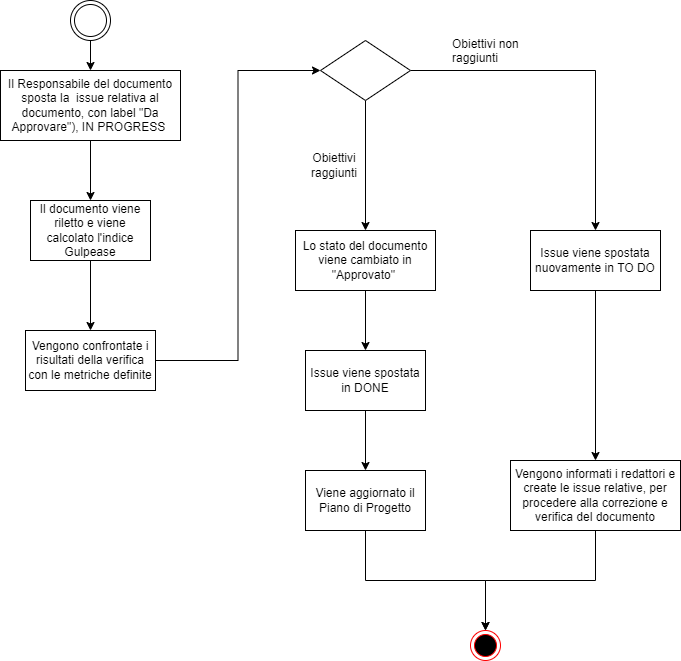
\includegraphics[scale=0.5]{Contenuto/Immagini/valid-documenti.png}
\caption{Attività di validazione dei documenti}
\end{figure}

\subsubsection{Validazione del codice}
La validazione del codice si compone di due attività principali:
\begin{itemize}
\item \textbf{Test di sistema e test di validazione};
\item \textbf{Collaudo}: attività di controllo che si svolge con la presenza di un committente, durante la Revisione di Accettazione. Dimostra la conformità del prodotto software secondo quanto promesso da contratto nei casi d’uso e nei requisiti espressi nell’\AdR ;
\end{itemize}

Il processo di validazione del codice prevede le seguenti attività:
\begin{itemize}
\item pianificazione e tracciamento dei test da eseguire sul codice prodotto;
\item esecuzione dei test;
\item controllo dei risultati, dove viene verificato se il sistema soddisfi i requisiti.
\end{itemize}

\paragraph{Test di validazione}
I test di validazione sono fondamentali per stabilire con certezza se si sta rispettando
quanto dichiarato nel contratto con il proponente. Essi coinvolgono l'intero prodotto e vengono eseguiti con la presenza dei committenti. Verifica il prodotto e, in particolare,
il soddisfacimento del cliente. Il superamento del test di validazione garantisce che il software è pronto per essere rilasciato.

\paragraph{Tracciamento}
Il tracciamento è una parte fondamentale nel processo di esecuzione dei test. Con un buon tracciamento si riesce a confermare il pieno rispetto e soddisfacimento di tutti i requisiti e della corretta implementazione di tutte le funzionalità.


